\documentclass{article}
\usepackage[utf8]{inputenc}
\usepackage{amsmath}
\usepackage[linesnumbered,ruled,vlined]{algorithm2e}\usepackage[T1]{fontenc}
\usepackage{pgfplots}
\usepackage{chngpage}
\usepackage{textcomp}
\usepackage{url}
\usepackage{booktabs}
\usepackage{subcaption}

\setlength\parindent{0pt}


\newcommand{\shellcmd}[1]{\\\texttt{\footnotesize\$ #1}\\}
\pgfplotsset{
  compat=newest,
  xlabel near ticks,
  ylabel near ticks
}

\newcommand\mycommfont[1]{\footnotesize\ttfamily\textcolor{blue}{#1}}

\title{INF6953G: Lab 3 \\Scaling Databases \\and Implementing Cloud Patterns}
\author{
    Foutse Khomh \\
    S. Amirhossein Abtahizadeh \\
    D\'{e}partement G\'{e}nie Informatique et G\'{e}nie Logiciel \\
    \'{E}cole Polytechnique de Montr\'{e}al, Qu\'{e}bec, Canada \\
    \texttt{foutse.khomh[at]polymtl.ca} \\
    \texttt{a.abtahizadeh[at]polymtl.ca}\\
    {} \\
    Le An, Alexandre Courouble, Mahdis Zolfagharinia
}

\date{24\textsuperscript{th} March, 2016}

\begin{document}
\maketitle



\section{What were the results of comparing MySQL to MySQL Cluster. Were any of the results surprising, why or why not?}\label{Q1}

For the sake of comparing MySQL to MySQL Cluster, we set up both databases on AWS EC2 t2.micro instances. The MySQL database was installed on a signle node, while the cluster was setup on a set of four different instances. The first instance would hold the Master and the MySQL nodes while the last three would host the data nodes. We were able to benchmark both databases using Sysbench.

 The following graphs show the performance of both MySQL and MySQL cluster for 1, 2, 4, 8, 16, 32, 64 threads. The first graph shows the performance for 5000 requests while the second show the performance for 10000 requests. Surprisingly, the standard, single node, MySQL database performed much better than the MySQL cluster. This is due to the fact that the cluster looses a lot of time retrieving its data in the different node, while the single MySQL database has its data stored locally. 
 
 
 
  % graphs go here
 % graphs go here
  % graphs go here
   % graphs go here
    % graphs go here
     % graphs go here
      % graphs go here
       % graphs go here

The following table display the results of our benchmarking process. As you can see, we ran each thread and each request for 5 time. 

\begin{table}[]
	\centering
	\caption{Standard MySQL database for 5,000 and 10,000 requests}
	\label{my-label}
	\begin{tabular}{@{}ccccccc@{}}
		\toprule
		Threads & RUN 1   & RUN 2   & RUN 3   & RUN 4   & RUN 5   & Average      \\ \midrule\midrule
		1       & 18.2 & 17.4  & 17.1 & 17.5 & 17.5 & 17.5 \\
		2       & 13.4   & 12.3   & 12.2 & 12.2 & 12.7 & 12.5 \\
		4       & 9.9  & 9.4  & 9.5   & 9.5  & 9.5  & 9.6  \\
		8       & 7.7  & 7.4   & 7.6  & 7.5  & 7.5  & 7.5  \\
		16      & 7.2  & 7.2  & 7.1  & 7.2   & 7.5  & 7.2  \\
		32      & 7.5  & 7.5  & 7.3  & 7.7  & 7.6  & 7.5  \\
		64      & 7.9   & 7.9  & 7.7   & 7.8  & 7.9   & 7.8  \\\midrule
		1       & 34.8 & 34.2 & 35.2 & 35.1   & 35.1 & 34.9 \\
		2       & 24.6 & 25.0 & 25.0 & 26.0 & 24.3 & 24.9   \\
		4       & 18.6 & 19.5 & 19.2 & 19.5 & 19.1 & 19.2 \\
		8       & 15.5 & 15.5 & 15.4 & 15.3 & 15.2 & 15.4 \\
		16      & 14.6 & 14.5 & 14.3  & 14.3 & 14.5 & 14.4  \\
		32      & 15.2 & 15.1 & 15.2 & 14.8 & 15.2  & 15.1  \\
		64      & 16.1 & 15.8 & 15.7 & 15.6 & 15.5 & 15.7 \\ \bottomrule
	\end{tabular}
\end{table}




\begin{table}[]
	\centering
	\caption{MySQL Cluster database for 5,000 and 10,000 requests}
	\label{my-label}
	\begin{tabular}{@{}ccccccc@{}}
		\toprule
		Threads & RUN 1    & RUN 2   & RUN 3   & RUN 4  & RUN 5  & Average      \\ \midrule\midrule
		1       & 173.2 & 172.9 & 173.7 & 174.7 & 173.5 & 173.6 \\
		2       & 89.5  & 89.3  & 91.7  & 89.1  & 90.6  & 90.1  \\
		4       & 51.4  & 50.6  & 50.4  & 49.9  & 50.9  & 50.7  \\
		8       & 37.8  & 33.8  & 34.4  & 34.4  & 32.4  & 34.6  \\
		16      & 31.5  & 35.8  & 33.0  & 28.9  & 29.2  & 31.7  \\
		32      & 33.4  & 29.9  & 30.1  & 37.7  & 38.3  & 33.9   \\
		64      & 96.3  & 103.1 & 93.9  & 93.5  & 90.1  & 95.4  \\\midrule
		1       & 347.2  & 345.8 & 347.6 & 346.3 & 345.6 & 346.5 \\
		2       & 179.8 & 179.3  & 178.6 & 178.5 & 178.5 & 178.9 \\
		4       & 102.7 & 102.8 & 102.7 & 102.6 & 102.9 & 102.7 \\
		8       & 72.4  & 76.2  & 67.1   & 65.7   & 64.6  & 69.2  \\
		16      & 55.4  & 66.8  & 52.4  & 58.7  & 53.9  & 57.46  \\
		32      & 72.7  & 67.1  & 65.9  & 68.1  & 76.7  & 70.1  \\
		64      & 163.2 & 177.5 & 201.6 & 194.4 & 173.9 & 182.1  \\ \bottomrule
	\end{tabular}
\end{table}

\section{When and why should we use the Gatekeeper and Competing Consumers Patterns?}\label{Q2}

The Competing Consumer Pattern is a cloud pattern that is meant to assure stability and availability for variable amount of requests. This pattern is a great scalable solution for an application with a highly variable workload. 

The Gatekeeper pattern is a pattern that has for purpose to keep sensitive information safe. We should use this pattern to prevent malicious user from injecting wrongful SQL commands to our database. 

\section{Describe your solutions to implement the two Cloud patterns strategies.}\label{Q3}
\subsection{Competing Consumers pattern}
\subsubsection{Overview}

\begin{figure}[t]
    \centering
        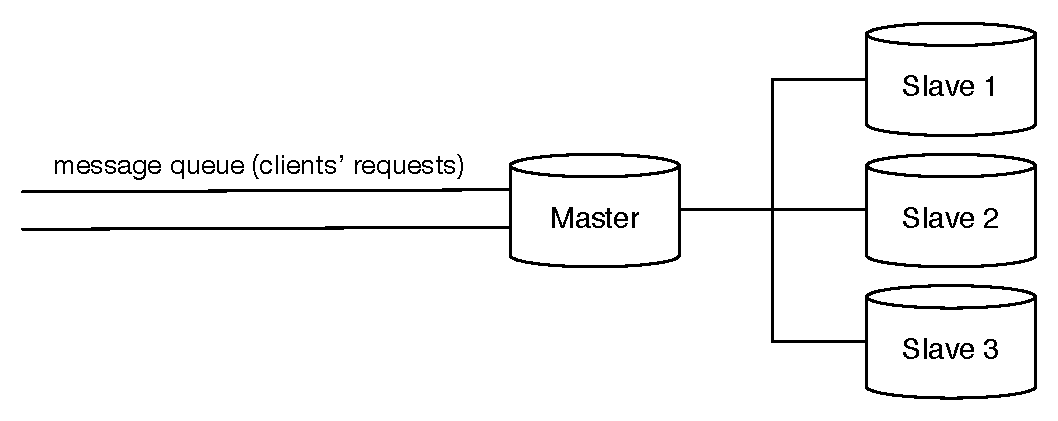
\includegraphics[width = 10cm]{images/CCP.pdf}
    \caption{Architecture of the servers that implement the Competing Consumers pattern.}
    \label{fig:arch1}
\end{figure}


We use four AWS t2.micro instances to build the server side of the \emph{Competing consumers pattern}. We install MySQL in all of the four instances. We configure the instances as a cluster, where one instance (the \emph{master node}) receives queries from clients and distributes them either to itself or to the other three instances (\emph{slave nodes}). The Competing Consumers pattern only handles \texttt{INSERT} SQL queries. After inserting a client request into the specific instance (referred as to \emph{data node}), the master node will reply the client with a message (\emph{e.g,} ``Data inserted into Slave1'').
Figure \ref{fig:arch1} illustrates the architecture of the servers, which implements the Competing consumers pattern.\\

In the rest of this section, we elaborate three key points of the implementation of this pattern in terms of the data nodes' configuration, master node's implementation, and socket connection. Our source code in Java can be found at: \url{https://goo.gl/Ln8InQ}.

\subsubsection{Configuration of data nodes}
We load \emph{Sakila} database into the 4 data nodes. The master node is responsible to balance work loads among the 4 data nodes, \emph{i.e.,} distributing and sending queries to itself or to the slave nodes.

\subsubsection{Implementation of the master node}\label{master-node}
For each client request, the master node will receive a string through the socket connection. The client request string contains the client identifier and her SQL request statement, an example of which is shown as follow:\\

\texttt{200a3b9b-17a1-4808-b1ba-54d159ea4108+2006||INSERT INTO film (title, description, release\_year, language\_id) VALUES (\textquotesingle sample\_movie\textquotesingle, \textquotesingle This is just a test\textquotesingle, 2016, 1)}\\

In the request, the client identifier and the SQL statement are separated by \texttt{||}. The master node parse the all letters and numbers (\emph{i.e.,} \texttt{[0-9a-z]}) in the client identifier to convert each of these characters to an ASCII decimal number and add all ASCII decimal numbers up. The result is noted as $DigitSum$. As there are 4 data nodes in the cluster, to balance the workload in these nodes, we divide $DigitSum$ by the number of data nodes (\emph{i.e.,} 4) and calculate the remainder, noted as $Rem$ (\emph{i.e.,} $DigitSum\%4=Rem$). $Rem$ is an integer ranged from 0 to 3. The master node will assign the request (by sending the SQL statement), where $Rem=0$, to itself; the request, where $Rem=1$, to slave node \#1; the request, where $Rem=2$, to slave node \#2; and the request, where $Rem=3$, to slave node \#3.\\

We use Java Database Connectivity (JDBC) API to send MySQL queries from the master node to data nodes. We configure the port 3306 for the MySQL communication among the 4 data nodes.

\subsubsection{Socket connection}
We leverage a message queue to to build a communication channel between clients and data servers. When a client's request has passed through the message queue, we will receive this request, concatenate the client's UID with its \texttt{INSERT} request statement, and send it to the master node by the socket connection.\\

In the socket connection, on the one hand, the client program establishes a socket connection object, which initialize a \texttt{DataOutputStream} object and a \texttt{DataInputStream} object. The client uses the \texttt{DataOutputStream} object to send the request (the client's UID + a SQL statement) to the master node, while the client uses the the \texttt{DataInputStream} to receive the response sent back by the master node.

On the other hand, the master node acts as the socket server, which runs a dead loop in order to wait for clients' requests. The master node uses a \texttt{DataInputStream} object to receive socket packets. One packet represents a client's request. The master node converts each of the packets into a \texttt{String} object (\emph{i.e.,} a request), then applied the mechanism described in Section \ref{master-node} to decide the request's priority and send it to the corresponding data node. Once a request is well inserted into the data node, the master node will reply to the client through a \texttt{DataOutputStream} object.\\

Similar to the real web environment, if there is a socket connection error, the client will receive an error message. Then, the client can decide whether to re-send a request to the master node.

\subsection{Gatekeeper pattern}
\subsubsection{Overview}

\begin{figure}[t]
    \centering
        \includegraphics[width = \columnwidth]{images/gatekeeper.pdf}
    \caption{Architecture of the servers that implement the Gatekeeper pattern.}
    \label{fig:arch2}
\end{figure}

We use 3 AWS t2.micro instances to build the server side of the \emph{Gatekeeper} pattern. The first instance refers as to the \emph{gatekeeper}, which filters out malicious information from all clients' requests. The second instance refers as to the \emph{trusted host}, which receives safe requests from the gatekeeper and send them to the database. The third instance refers as to the \emph{sensitive data node}, which handles clients' requests and send the result back to the trusted host. To ensure the confidentiality of the database, the sensitive data node can be only reached by the trusted host. And the trusted host can be only reached by the gatekeeper and the sensitive data node. Therefore, one client's request targeted to the sensitive data node will pass through the gatekeeper, trusted host, and handled by the the sensitive data node; then the results will be sent back from the sensitive data node through the trusted host and the gatekeeper to the client. Figure \ref{fig:arch2} illustrates the architecture of the servers, which implements the Gatekeeper pattern.\\

In the rest of this section, we elaborate three key points of the sensitive data node's configuration, the trusted host's configuration and implementation, and the gatekeeper's implementation. Our source code in Java can be found at: \url{https://goo.gl/Ges57T}.

\subsubsection{Configuration of the sensitive data node}
We configure the security rules (through AWS security group) and allow the instance of the sensitive data node to only accept the inbound TCP requests from the IP of the trusted host through the port 3306. Thus, other machines cannot directly send queries to the sensitive database.

\subsubsection{Configuration and implementation of the trusted host}
We configure the security rules and allow the instance of the trusted host to only accept the inbound requests from the IP of the gatekeeper through the port of 6666. Thus, only the gatekeeper can directly send a query to the trusted host, which can then transfer the query to the sensitive database.\\

The trusted host applies a socket connection to exchange data with the gatekeeper. In this connection, the trusted host acts as a socket server, which runs a dead loop to wait for the gatekeeper's queries. While the gatekeeper acts as a socket client, which sends safe SQL queries to the trusted host and sends back the responses to clients.\\

The trusted host uses JDBC API\footnote{\url{https://docs.oracle.com/javase/8/docs/technotes/guides/jdbc/}} to send MySQL queries, which are received from the gatekeeper, to the sensitive data node. The JDBC API will wait and receive the responses from the sensitive data node, and send them back to the gatekeeper.

\subsubsection{Implementation of the gatekeeper node}
The gatekeeper node receives \texttt{SELECT} or \texttt{INSERT} requests from clients. As in Section \ref{master-node}, the gatekeeper node parses a client request to extract her UID and the SQL query. It considers the requests, in which the UID with the first character as letters (\emph{i.e.,} \texttt{[a-z]}, ASCII code from 97 to 122) as safe requests, and will transfer them to the trusted host. Other requests are considered as malicious requests, and will be rejected by the gatekeeper node. \\

To communicate with clients, there is another socket connection between the gatekeeper node and the client program. In this socket connection, the gatekeeper node acts as a socket server, while the client program acts as a socket client.


\section{Describe the implementation of multi-threaded application scenarios.}\label{Q4}

\section{What were the results of comparing the patterns in terms of performance? Were any of the results surprising, why or why not?}\label{Q5}

\subsection{Setup}
We intend to compare the performance between the Competing Consumers pattern and Gatekeeper pattern. We use the following scenario to evaluate the performance of the pattern applications. 

\begin{itemize}
\item We simulate respectively 25, 50, 75, and 100 concurrent clients for the scenario. The GlassFish server is deployed in an AWS instance, which connects with the master node (in the Competing Consumers pattern) and with the gatekeeper node (in the Gatekeeper pattern).
\item For the Competing Consumers pattern, each of the clients send 5 \texttt{SELECT} queries to the database, then wait for 5 seconds; she send 100 \texttt{SELECT} queries to the database, then wait for 5 seconds; she finally send 5 \texttt{INSERT} queries to the database. For the Gatekeeper pattern, the clients only send \texttt{INSERT} queries to the database.
\item We repeat the scenario 5 times for each number of clients.
\end{itemize}

We use the application execution time to measure their performance. The lower the execution time indicates the higher performance of the pattern application.


\begin{table}[t]
    \centering
    \caption{Application execution time of the Competing Consumers pattern.}
    \label{tab:ccp_performance}
    \begin{tabular}{|c|r|r|r|r|r|r|}
        \hline
        \textbf{\# of clients} & \textbf{Run1} & \textbf{Run2} & \textbf{Run3} & \textbf{Run4} & \textbf{Run5} & \textbf{Average}\\ \hline
        25 & 207 & 208 & 206 & 203 & 207 & 206.2 \\ \hline 
        50 & 404 & 403 & 406 & 410 & 416 & 407.8 \\ \hline
        75 & 602 & 604 & 608 & 604 & 605 & 604.6 \\ \hline
        100 & 795 & 801 & 808 & 834 & 806 & 808.8 \\ \hline
	\end{tabular}
\end{table}

\begin{table}[]
    \centering
    \caption{Application execution time of the Gatekeeper pattern.}
    \label{tab:gatekeeper_performance}
    \begin{tabular}{|c|r|r|r|r|r|r|}
        \hline
        \textbf{\# of clients} & \textbf{Run1} & \textbf{Run2} & \textbf{Run3} & \textbf{Run4} & \textbf{Run5} & \textbf{Average}\\ \hline
        25 & 204 & 205 & 203 & 205 & 205 & 204.4 \\ \hline 
        50 & 405 & 403 & 403 & 402 & 402 & 403 \\ \hline
        75 & 603 & 605 & 605 & 605 & 650 & 613.6 \\ \hline
        100 & 793 & 805 & 806 & 806 & 805 & 803 \\ \hline
	\end{tabular}
\end{table}

\begin{figure}[t]
    \centering
        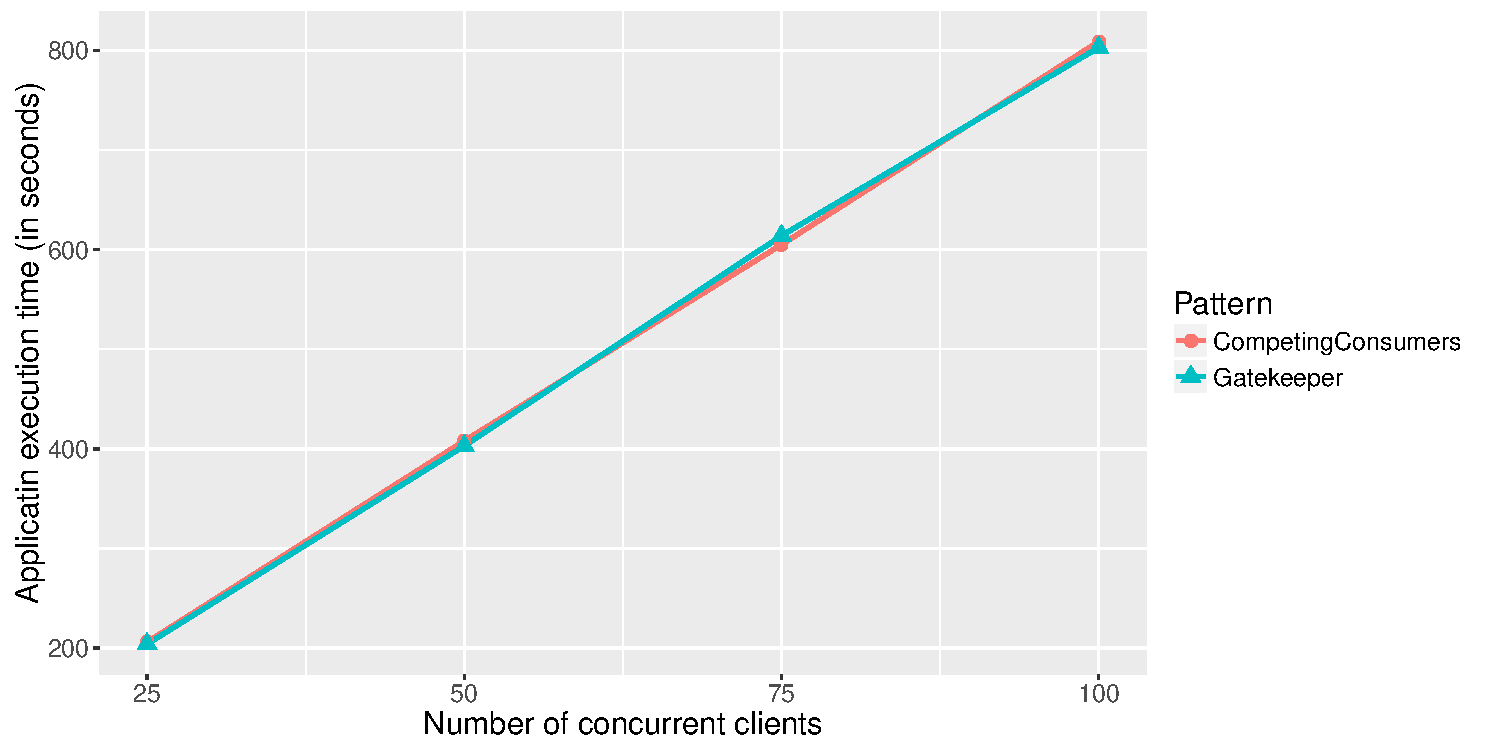
\includegraphics[width = \columnwidth]{images/performance.pdf}
    \caption{Comparison of the execution time (in seconds) of the Competing Consumers pattern against the Gatekeeper pattern.}
    \label{fig:performance}
\end{figure}


\subsection{Results}
Table \ref{tab:ccp_performance} and Table \ref{tab:gatekeeper_performance} show the execution time of the Competing Consumers pattern and the Gatekeeper pattern according to the scenario. Figure \ref{fig:performance} illustrates the average execution time (in the 5 runs) of the two patterns. We observe that the execution time tends to linearly increase with the increase of the clients. The two cloud design patterns have very similar execution time for each number of clients.\\

These results are not surprising, because for the two patterns, their scenario and concurrent clients are generated by the same machine. They also use the same GlassFish server to transform REST calls to the queries. Therefore, the two pattens need the same time to simulate concurrent client requests. 

In addition, the speed of the network connection between clients and data nodes is much slower than the response speed of data nodes.
Although there are four data nodes handling the SQL queries in the Competing consumers pattern, while there are only one data node handling the SQL queries in the Gatekeeper pattern, the total network connection time between clients and data nodes decides the execution time of our cloud service application.

Hence, when the network connection becomes the bottleneck of the speed of the service, higher number of concurrent clients needs higher number of total requests, which requires a larger amount of time to be executed.

\section{What were the results of measuring energy consumption in the two cloud design patterns?}\label{Q6}
\subsection{Setup}
We also intend to compare the energy consumption of the Competing Consumers patterns against the Gatekeeper pattern. We use the same scenario and the same numbers of clients as in Section \ref{Q5}.\\

We use a software-based energy measurement tool, PowerAPI \cite{noureddine2012preliminary}, to measure the energy consumption of the MySQL processes in terms of CPU in the data nodes. PowerAPI outputs the power of the subject process (in Watt) based on a certain sampling frequency. We use the frequency of 1 second to measure the power generated by the each MySQL process. We use the command line interface (CLI) of PowerAPI collect the CPU power with the frequency of 1 second as follow:

\texttt{./bin/powerapi modules procfs-cpu-simple monitor -{}-frequency 1000 \\-{}-apps mysqld}\\

Then, we use the following equation to calculate the energy consumed by the MySQL process (in Joule).

\begin{equation} \label{eq:energy}
E(J) = P(W) \times t(s)
\end{equation}

where $E(J)$ stands for the energy consumption in Joule, $P(W)$ stands for the power of the process in Watt, and $t(s)$ stands for the time spent during each power collection.\\

To ensure the precision of the energy consumption measurement, we start the PowerAPI CLI in each of the studied data nodes (four in the Competing Consumers pattern and one in the Gatekeeper pattern) before launching the pattern application. This approach would cause that PowerAPI runs one or two seconds earlier than the cloud pattern application. But according to our observation, PowerAPI can precisely evaluate the power generated by the subject process. Before launching a cloud pattern application, the PowerAPI always output 0 on the power generated by the data nodes in terms of the MySQL processes.

We stop the PowerAPI CLI in each of the studied data nodes after the a cloud application scenario has been accomplished.

Finally, we sum the energy consumed by the subject MySQL process in every second during the application's execution period to obtain the total energy consumed in a data node's CPU.


\begin{table}[t]
    \centering
    \caption{Energy consumption in the data nodes in terms of CPU for the Competing Consumers pattern.}
    \label{tab:ccp_energy}
    \begin{tabular}{|c|r|r|r|r|r|r|}
        \hline
        \textbf{\# of clients} & \textbf{Run1} & \textbf{Run2} & \textbf{Run3} & \textbf{Run4} & \textbf{Run5} & \textbf{Average}\\ \hline
        25 & 9.1 & 9.2 & 8.8 & 8.7 & 8.8 & 8.9 \\ \hline 
        50 & 17.1 & 17.3 & 17.4 & 16.6 & 17.1 & 17.1 \\ \hline
        75 & 27.8 & 27.3 & 27.4 & 27.0 & 25.1 & 26.9 \\ \hline
        100 & 29.3 & 30.3 & 26.0 & 29.3 & 28.5 & 28.7 \\ \hline
	\end{tabular}
\end{table}

\begin{table}[]
    \centering
    \caption{Energy consumption in the data node in terms of CPU for the Gatekeeper pattern.}
    \label{tab:gatekeeper_energy}
    \begin{tabular}{|c|r|r|r|r|r|r|}
        \hline
        \textbf{\# of clients} & \textbf{Run1} & \textbf{Run2} & \textbf{Run3} & \textbf{Run4} & \textbf{Run5} & \textbf{Average}\\ \hline
        25 & 0.4 & 0.9 & 0.3 & 0.3 & 0.4 & 0.5 \\ \hline 
        50 & 0.8 & 0.6 & 0.3 & 0.7 & 0.7 & 0.6 \\ \hline 
        75 & 0.9 & 0.7 & 0.9 & 1.0 & 2.0 & 1.1 \\ \hline 
        100 & 1.6 & 1.7 & 1.7 & 1.2 & 1.1 & 1.5 \\ \hline 
	\end{tabular}
\end{table}

\begin{figure}[t]
    \centering
        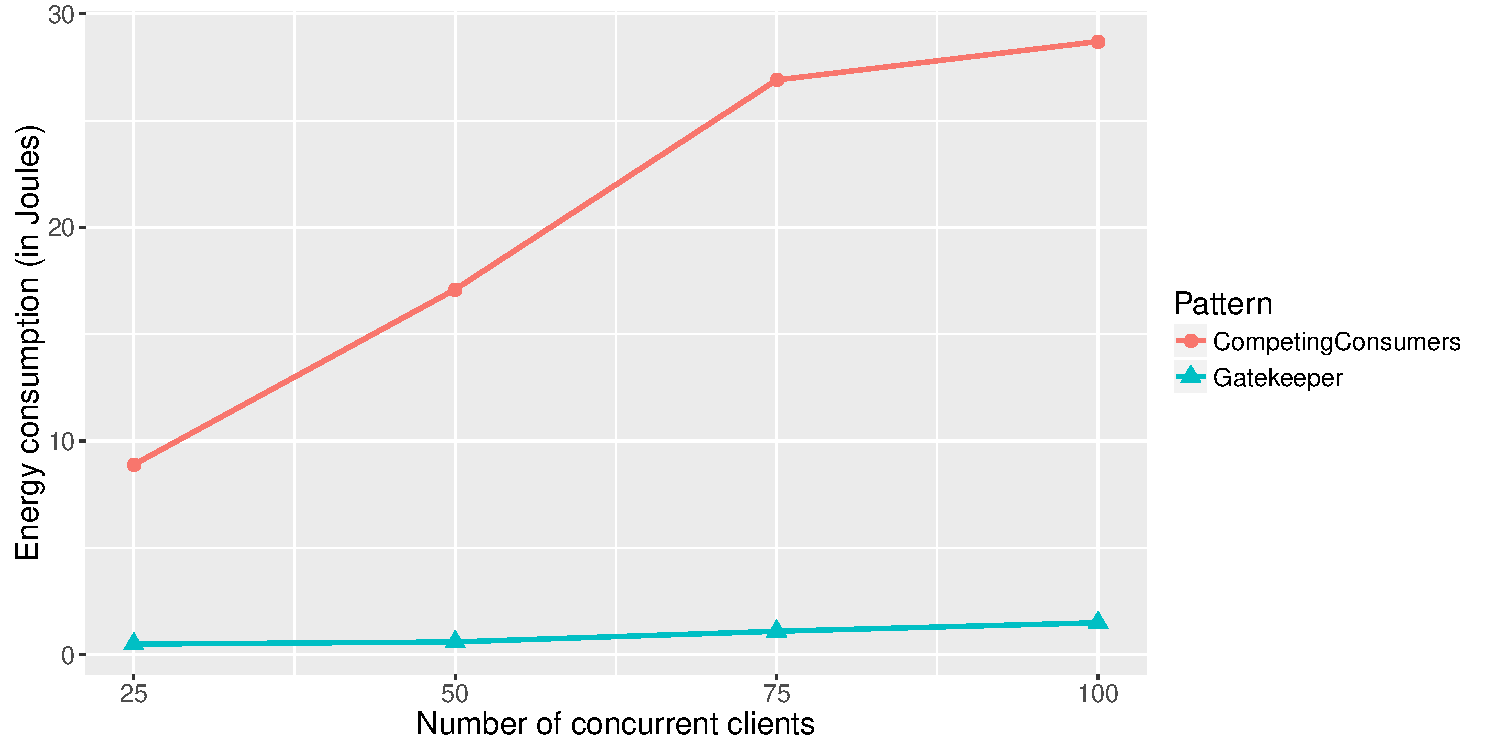
\includegraphics[width = \columnwidth]{images/energy.pdf}
    \caption{Comparison of the energy consumption (in Joules) of the Competing Consumers pattern against the Gatekeeper pattern.}
    \label{fig:energy}
\end{figure}


\subsection{Results}
Table \ref{tab:ccp_energy} and Table \ref{tab:gatekeeper_energy} show the data nodes' energy consumption in terms of CPU for the Competing Consumers pattern and the Gatekeeper pattern according to our scenario. Figure \ref{fig:energy} compares the average energy consumption in the data nodes' CPUs (in the 5 runs) between the two patterns.\\

We observe that the data nodes of the Competing Consumers pattern consume significantly more energy than the data node of the Gatekeeper pattern. Because we only use one data node in the Gatekeeper pattern, while we use four data nodes in the Competing Consumers pattern. In addition, in the Gatekeeper pattern, the gatekeeper node refuse all request in which the UID begins with a number. In other words, about half of the requests are not reached to the data node, but are rejected by the gatekeeper node.

In both cloud design patterns, the energy consumption tends to increase with the increase of the concurrent client numbers. In the Competing Consumers pattern, energy consumption increases linearly with the number of clients when the client number is from 25 to 75. But when the client number is from 75 to 100, the energy consumption only slightly increases. One explanation is that, based on the network connection capacity (among AWS instances) and the data nodes' MySQL processing capacity, the four data nodes in this pattern can handle up to $\frac{75\times100}{4}=1875$ requests per second. When the number of clients is more than 75, the network connection and the data nodes will reach their maximum capacity. Therefore, the increasing trend of the energy consumption tends to slow down with the increase of the number of clients. For the Gatekeeper pattern, the energy consumption tend to linearly increase with the increase of the number of clients. There is only a little difference of energy consumption between 25 clients and 50 clients in the Gatekeeper pattern, because Run \#2 of 25 clients is an outlier, which consume more than 100\% energy than other runs. In the future, we will eliminate outliers and use the median value of all runs to avoid this problem.

\section{Discussion and future work}
In this project, we experienced a lot of failures when using the GlassFish server. Especially, if we set the number of concurrent clients more than 250, the failure rate significantly increases. We tried to tune the configuration of the GlassFish server on the thread pool size, and also to optimize MySQL on maximum connection and maximum timeout. But we still met failures when the client number is large. In addition, as we observed the linear increasing trend of the execution time of our applications with the increase of the client number, we may need about two hours to run a scenario with 1000 clients. 5 runs with 1000 clients for both patterns would require about 10 hours. Therefore, 5 runs for all client numbers would require 18.5 hours. If we experienced failures, the required time to accomplish the whole experiment will be even longer and unpredictable. Thus, with the limited time, we reduce the numbers of clients to 25, 50, 75, and 100. Our experimental client numbers may not represent concurrent requests received by a cloud service in the real-life. But our experiment can show preliminary results on the comparison of Competing Consumers pattern against Gatekeeper pattern in terms of performance and energy consumption. In order to show insight to cloud provider on the performance and energy consumption of cloud patterns, we need:\\

\begin{itemize}
\item Deploy our cloud pattern applications in the machines with better performance than AWS t2.micro.
\item Consider to replace the GlassFish server with newer resolutions to obtain a higher stability. 
\item Adjust our experimental scenario. Because in the real-life, a client cannot generate 100 requests without any interval like a robot. In the future, we plan add some interval time to more closely simulate a client's consecutive queries. 
\item Optimize the performance metric. The total application execution time may not be the best metric to measure the performance of a cloud pattern. In the future, we need to measure the amount of time spent for each query from the it is sent from the client side until the client receives the response. Then we can calculate the average or median response time of all queries of all clients. This result can better reflect a cloud service's performance.
\item Improve the measurement of energy consumption. Although PowerAPI is a popularly used tool, it cannot fresh the power generated of a specific process with a high frequency. In the future, we need to compare the energy consumption results measured by a software-based tool with a hard-ware based tool. Another issue about the energy consumption is that not only CPU consumes energy when handling a SQL query. Other component in a machine, such as memory, network card also need energy to accomplish the query. In addition, as we use AWS's virtual machine to deploy our cloud pattern applications, PowerAPI's output may not reflect the real energy consumption of the physical machines. This gives us another reason to compare the results yielded by PowerAPI and other hardware-based energy measurement tool. To apply hardware-based energy measurement tool the energy consumption, we also need to deploy the cloud applications in our own physical machines. 
\end{itemize}

\bibliographystyle{IEEEtran}
\bibliography{references}

\end{document}